
\documentclass[a4paper]{article}

\usepackage[utf8]{inputenc}

\usepackage{geometry}

\geometry{legalpaper, margin=1in}

\usepackage[T1]{fontenc}

\usepackage{algorithm}

\newcommand\tab[1][1cm]{\hspace*{#1}}

\usepackage{graphicx}



\title{SDD : TP 2}

\author{Mathieu Boutin - Jérémy Morceaux}

\begin{document}
\maketitle
\section{Présentation générale}
- Ce TP a pour but de créer les fonctions de base permettant de manipuler des piles et des files qui seront utiles pour le prochain TP. A l'aide de ses fonctions, on inverse une pile grâce à une file supplémentaire en vidant la pile dans la file, puis inversement, en vidant la file dans la pile.
\\
\\
\begin{center}
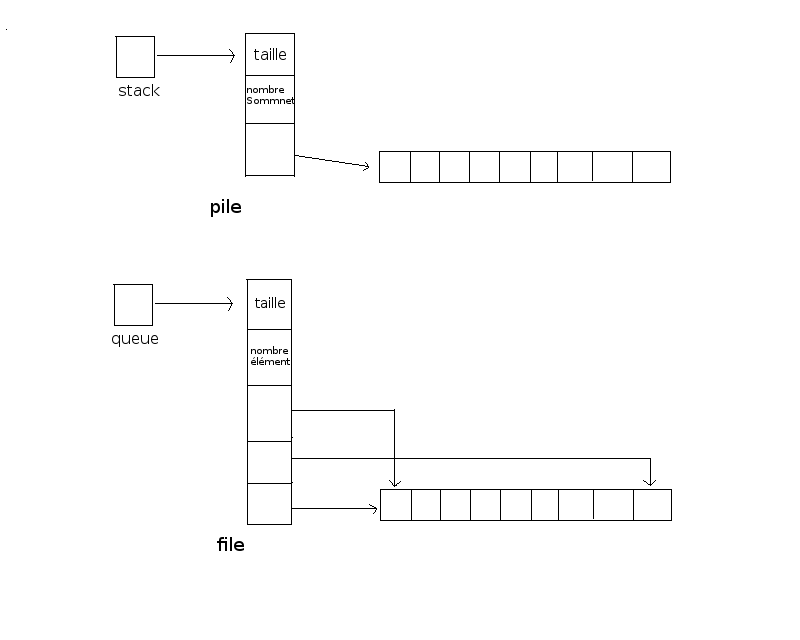
\includegraphics[scale=0.4]{Schema_base.png}

Schéma de base
\end{center}
\underline{Structure des fichiers de pile : prenons par exemple une pile de taille n}
\\
\\
1ère ligne fichier : <taille de la pile>
\\
2ème ligne du fichier: $valeur_{0}$ $valeur_{1}$  ... $valeur_{n-1}$
\\
\\
- Les fichiers sources se trouvent dans le dossier \textbf{src}. Les fonctions relatives aux piles sont dans le fichier \textbf{ZZ\_stack.c} et celles des files sont dans le fichier \textbf{ZZ\_queue.c}. Les entêtes sont dans le fichier \textbf{include}.

\section{Détail de chaque fonction}

\subsection{initStack}
\underline{Lexique :}

\begin{itemize}

\item Paramètre(s) de la fonction  

\begin{itemize}

\item size est la taille de la pile.

\item errorCode est un pointeur sur un entier qui indique si la fonction s'est bien déroulée.

\end{itemize}

\item Variable(s) locale(s)

\begin{itemize}

\item p est un pointeur de la pile.
\end{itemize}

\end{itemize}

\underline{Programme commenté :}
\begin{center}
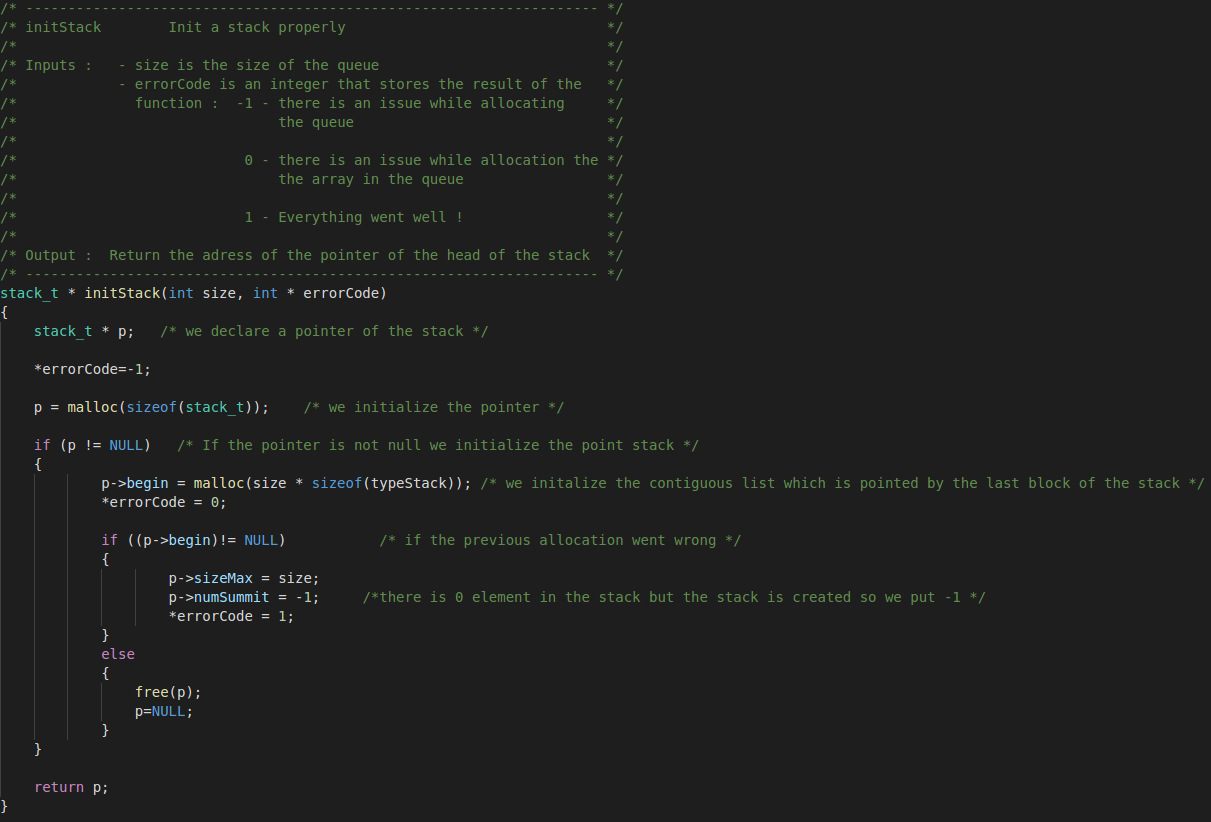
\includegraphics[scale=0.4]{initStack.png}

initStack
\end{center}
\subsection{initStackFromFile}
\underline{Lexique :}

\begin{itemize}

\item Paramètre(s) de la fonction  

\begin{itemize}

\item fileName est le nom du fichier contenant la pile
\item errorCode est un pointeur sur un entier qui indique si la fonction s'est bien déroulée.

\end{itemize}
\item Variables(s) locale(s)

\begin{itemize}

\item stack est le pointeur de la pile.
\item size contient la taille de la pile.
\item codeE\_init errorCode est un pointeur sur un entier qui indique si la fonction init s'est bien déroulée.
\item codeE\_push errorCode est un pointeur sur un entier qui indique si la fonction push s'est bien déroulée.
\item issue indique s'il y a eu un problème pendant un push.
\item file est le flux du fichier.
\item value contient une valeur à mettre dans la pile.

\end{itemize}
\end{itemize}

\underline{Programme commenté :}
\begin{center}
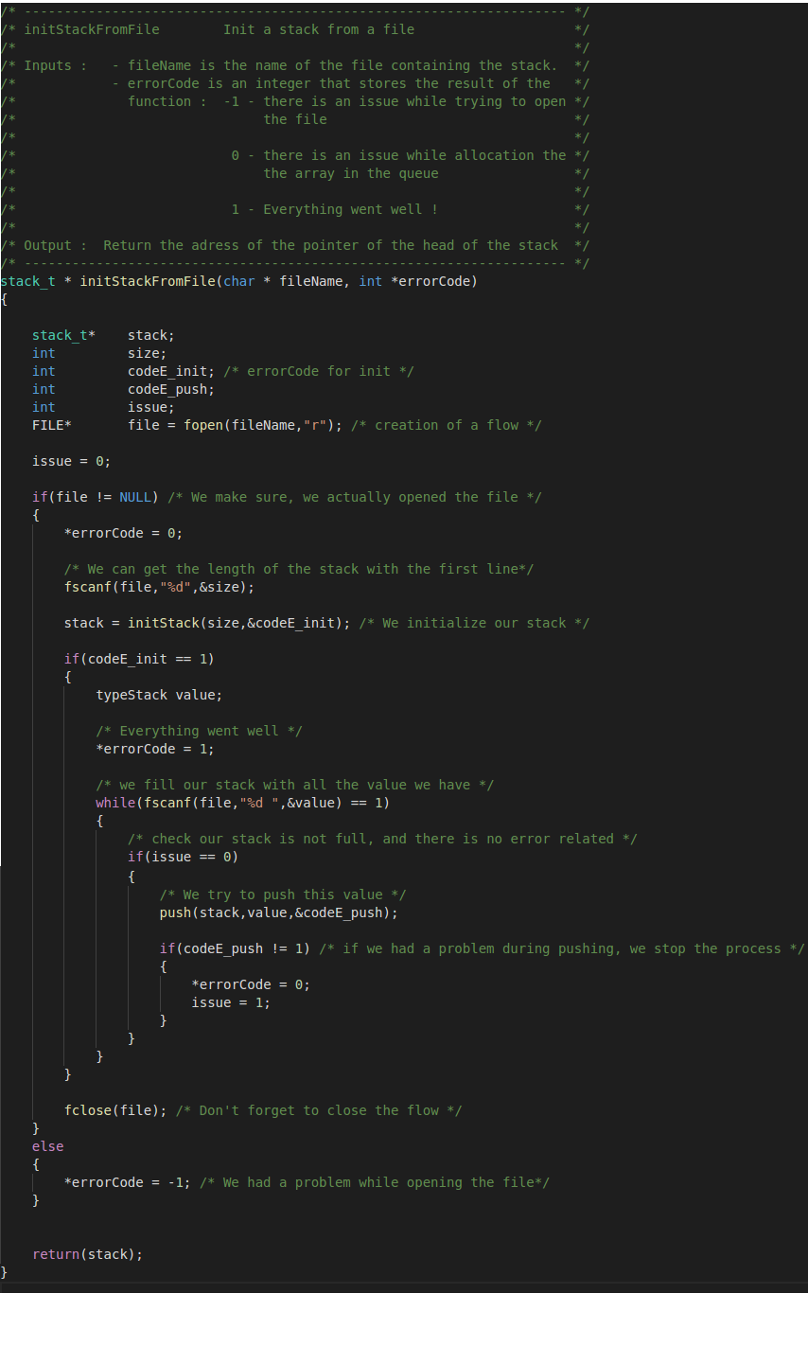
\includegraphics[scale=0.4]{initStackFromFile.png}

initStackFromFile
\end{center}
\subsection{printStack}
\underline{Lexique :}

\begin{itemize}

\item Paramètre(s) de la fonction  

\begin{itemize}

\item p est la tête fictive de la pile.

\end{itemize}
\item Variables(s) locale(s)  

\begin{itemize}

\item i permet de parcourir la pile.

\end{itemize}

\end{itemize}

\underline{Programme commenté :}
\begin{center}
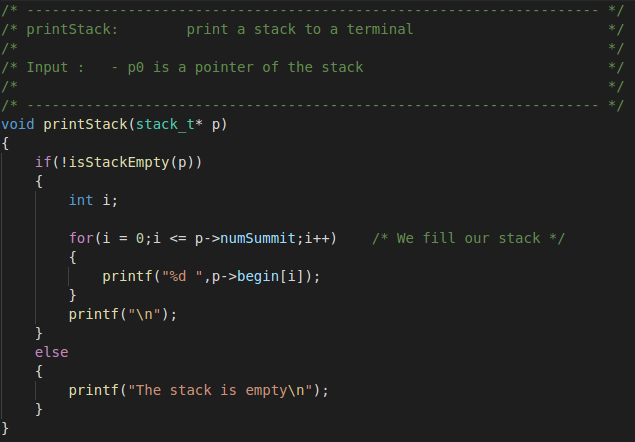
\includegraphics[scale=0.4]{printStack.png}

printStack
\end{center}
\subsection{freeStack}
\underline{Lexique :}

\begin{itemize}

\item Paramètre(s) de la fonction  

\begin{itemize}

\item p est la tête fictive de la pile.

\end{itemize}

\end{itemize}

\underline{Programme commenté :}
\begin{center}
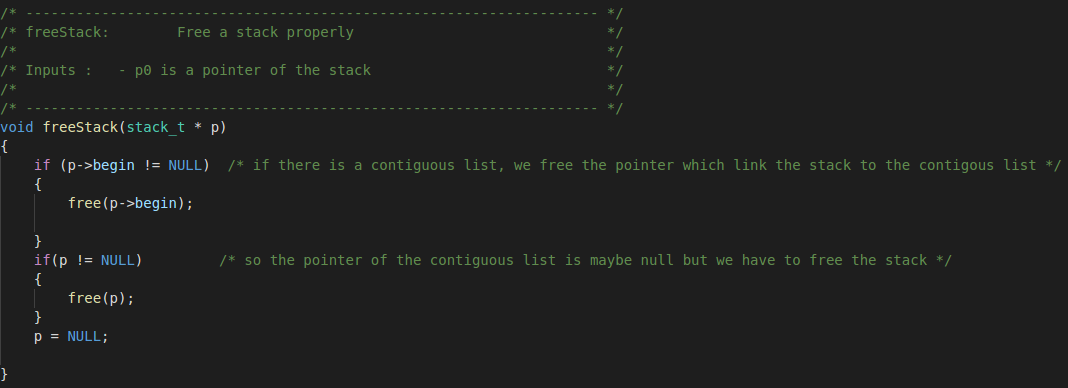
\includegraphics[scale=0.4]{freeStack.png}

freeStack
\end{center}
\subsection{isStackEmpty}
\underline{Lexique :}

\begin{itemize}

\item Paramètre(s) de la fonction  

\begin{itemize}

\item p est le pointeur de tête fictive de la pile.

\end{itemize}

\end{itemize}

\underline{Programme commenté :}
\begin{center}
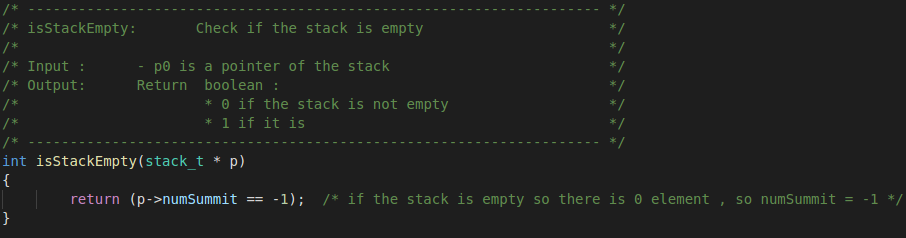
\includegraphics[scale=0.4]{isStackEmpty.png}

isStackEmpty\end{center}
\subsection{push}
\underline{Lexique :}

\begin{itemize}

\item Paramètre(s) de la fonction  

\begin{itemize}

\item p est le pointeur de tête fictive de la pile.

\item errorCode est un pointeur sur un entier qui indique si la fonction s'est bien déroulée.

\item v est la valeur que l'on veut mettre dans la pile.

\end{itemize}


\end{itemize}

\underline{Programme commenté :}
\begin{center}
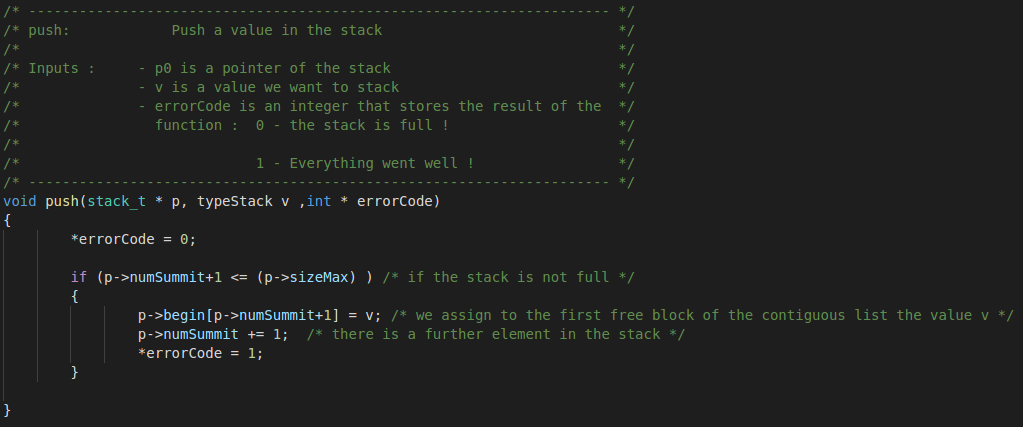
\includegraphics[scale=0.4]{push.png}

push
\end{center}
\subsection{pop}
\underline{Lexique :}

\begin{itemize}

\item Paramètre(s) de la fonction  

\begin{itemize}

\item p est le pointeur de tête fictive de la pile.

\item errorCode est un pointeur sur un entier qui indique si la fonction s'est bien déroulée.

\item v est la variable dans laquelle on va mettre l'élément que l'on dépile.

\end{itemize}
\end{itemize}
\underline{Programme commenté :}
\begin{center}
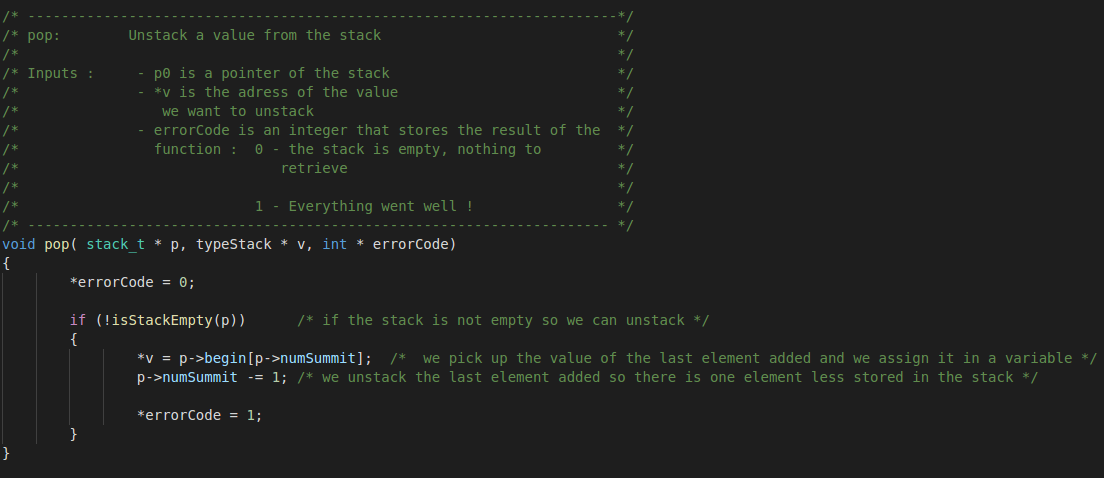
\includegraphics[scale=0.4]{pop.png}

pop
\end{center}
\subsection{initQueue}
\underline{Lexique :}

\begin{itemize}

\item Paramètre(s) de la fonction  

\begin{itemize}

\item size est la taille de la file.

\item errorCode est un pointeur sur un entier qui indique si la fonction s'est bien déroulée.
\end{itemize}
\item Variables(s) locale(s)  

\begin{itemize}

\item p0 est le pointeur vers la file qui sera retournée.

\end{itemize}
\end{itemize}
\underline{Programme commenté :}
\begin{center}
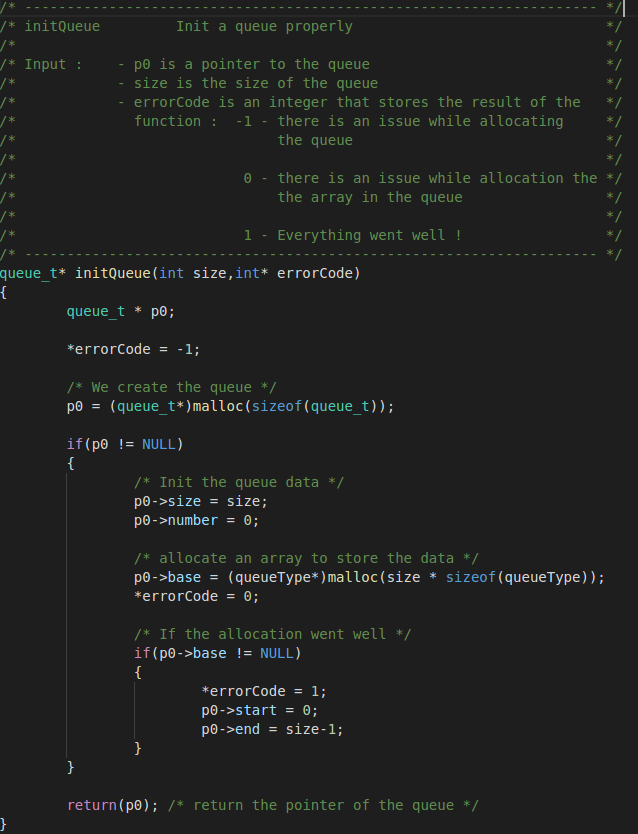
\includegraphics[scale=0.4]{initQueue.png}

initQueue
\end{center}
\subsection{enterQueue}
\underline{Lexique :}

\begin{itemize}

\item Paramètre(s) de la fonction  

\begin{itemize}

\item p0 est le pointeur de tête fictive de la file.

\item errorCode est un pointeur sur un entier qui indique si la fonction s'est bien déroulée.

\item element est l'élément que l'on veut insérer dans la file.

\end{itemize}
\end{itemize}
\underline{Programme commenté :}
\begin{center}
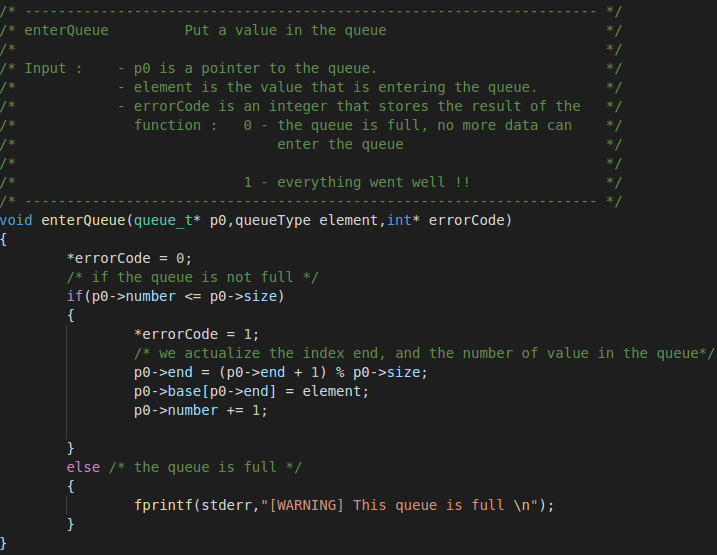
\includegraphics[scale=0.4]{enterQueue.png}

enterQueue
\end{center}
\subsection{leaveQueue}
\underline{Lexique :}

\begin{itemize}

\item Paramètre(s) de la fonction  

\begin{itemize}

\item p0 est le pointeur de tête fictive de la file.

\item errorCode est un pointeur sur un entier qui indique si la fonction s'est bien déroulée.

\end{itemize}
\item Variables(s) locale(s)  

\begin{itemize}

\item res est la variable qui contient l'élément qui sera défilé.

\end{itemize}
\end{itemize}
\underline{Programme commenté :}
\begin{center}
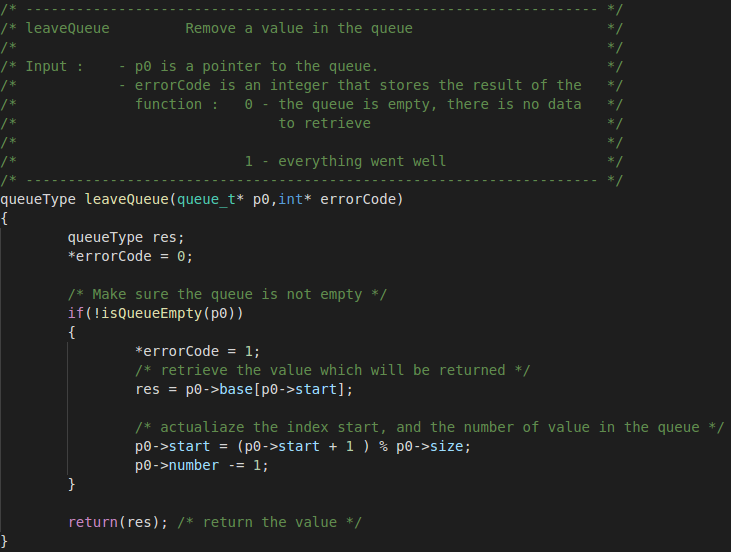
\includegraphics[scale=0.4]{leaveQueue.png}

leaveQueue
\end{center}
\subsection{isQueueEmpty}
\underline{Lexique :}

\begin{itemize}

\item Paramètre(s) de la fonction  

\begin{itemize}

\item p0 est le pointeur de tête fictive de la file.

\end{itemize}

\end{itemize}

\underline{Programme commenté :}
\begin{center}
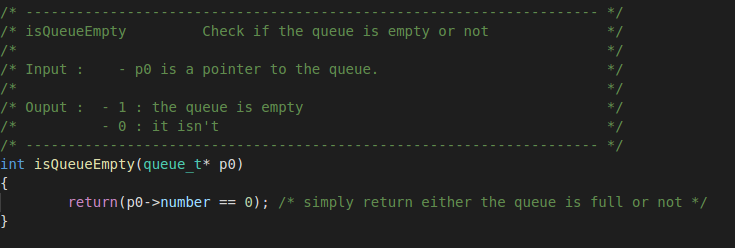
\includegraphics[scale=0.4]{isQueueEmpty.png}

isQueueEmpty
\end{center}
\subsection{freeQueue}
\underline{Lexique :}

\begin{itemize}

\item Paramètre(s) de la fonction  

\begin{itemize}

\item p0 est la tête fictive de la file.

\end{itemize}

\end{itemize}

\underline{Programme commenté :}
\begin{center}
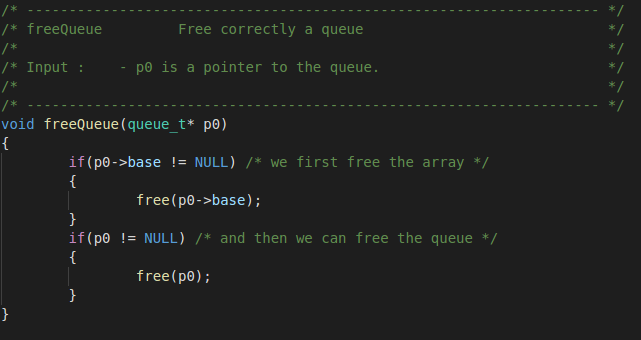
\includegraphics[scale=0.4]{freeQueue.png}

freeQueue
\end{center}
\subsection{printQueue}
\underline{Lexique :}

\begin{itemize}

\item Paramètre(s) de la fonction  

\begin{itemize}

\item p0 est la tête fictive de la file.

\end{itemize}
\item Variables(s) locale(s)  

\begin{itemize}

\item i permet de parcourir la file.

\end{itemize}
\end{itemize}
\underline{Programme commenté :}
\begin{center}
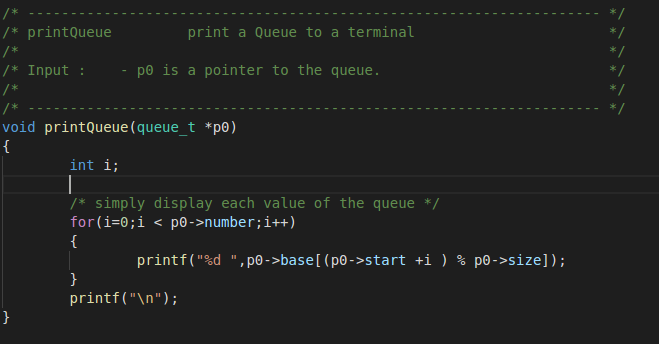
\includegraphics[scale=0.4]{printQueue.png}

printQueue
\end{center}
\subsection{main}
\underline{Lexique :}

\begin{itemize}
\item Variables(s) locale(s)  

\begin{itemize}

\item queue pointe vers la pile.
\item stack pointe vers la file.
\item errorCode est un pointeur sur un entier qui indique si une fonction s'est bien déroulée.
\item fileName contient le nom du fichier contenant la pile.
\item i permet de vider la pile pour remplir la file et inversement.
\item numberSummit contient le nombre de valeur dans la pile.
\item empty et full sont des variables permettant de stopper les boucles for au cas où il y est une erreur ( une pile vide ou pleine, de même pour la file).
\end{itemize}
\end{itemize}
\underline{Programme commenté :}
\begin{center}
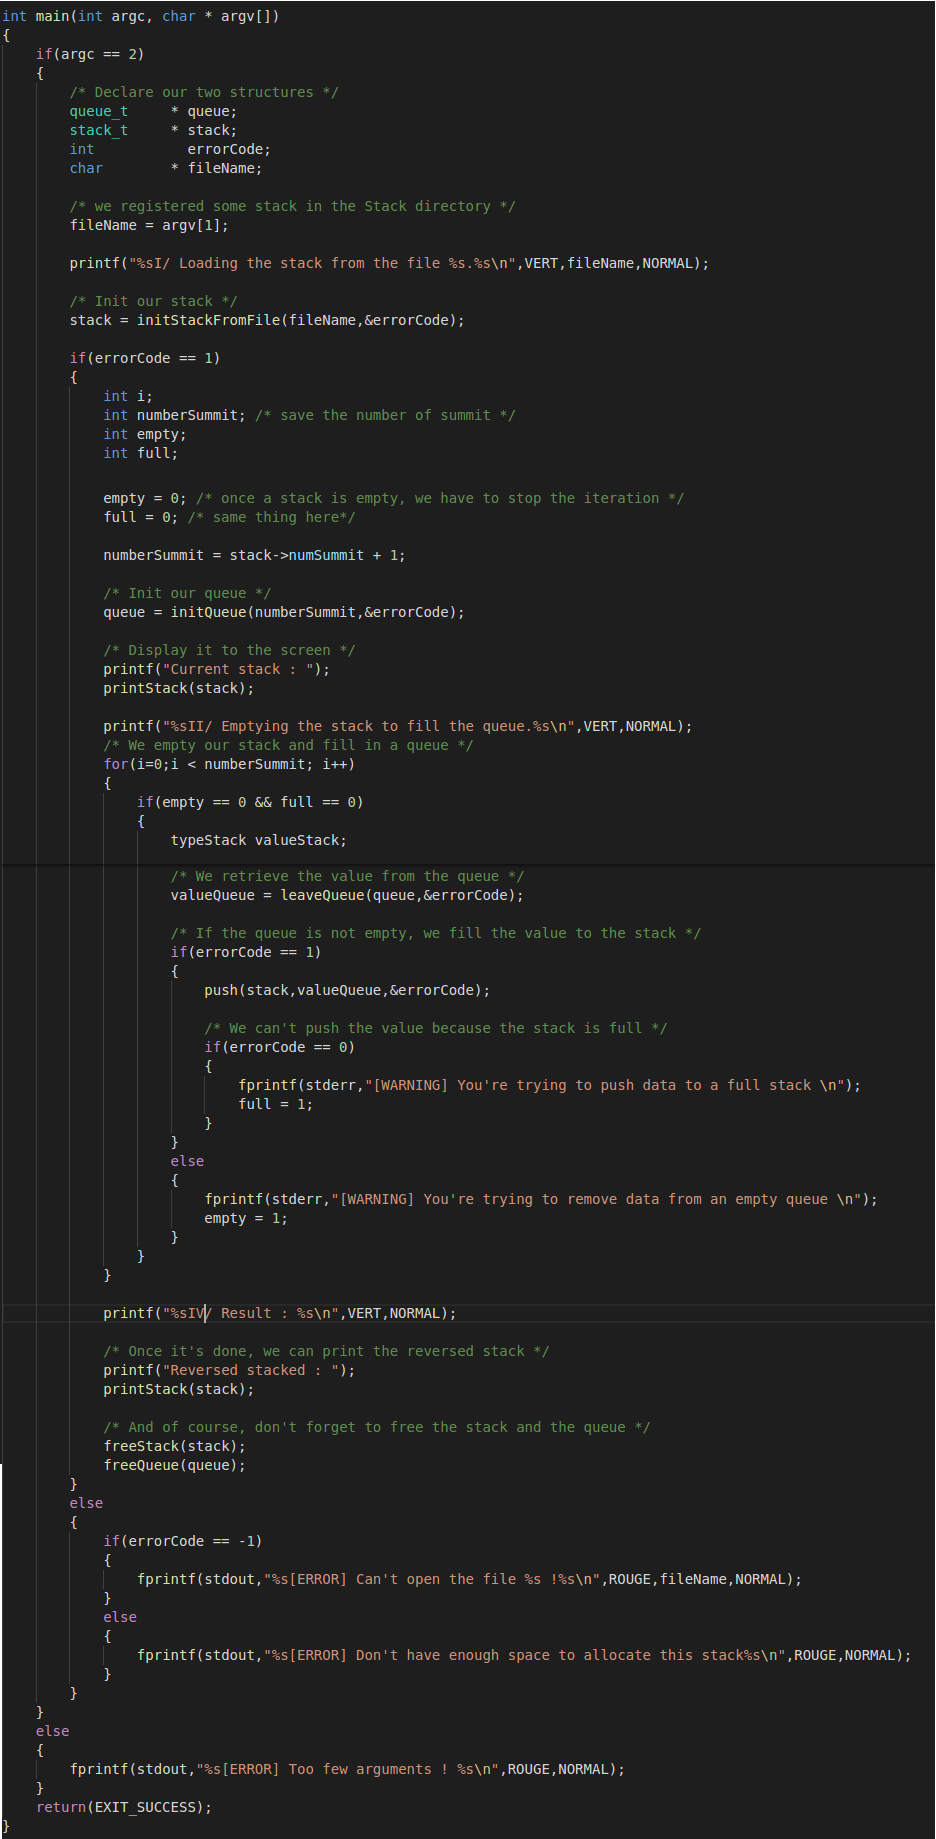
\includegraphics[scale=0.4]{main.png}

main
\end{center}
\section{Compte rendu d'exécution}

\underline{Makefile :}
\begin{center}
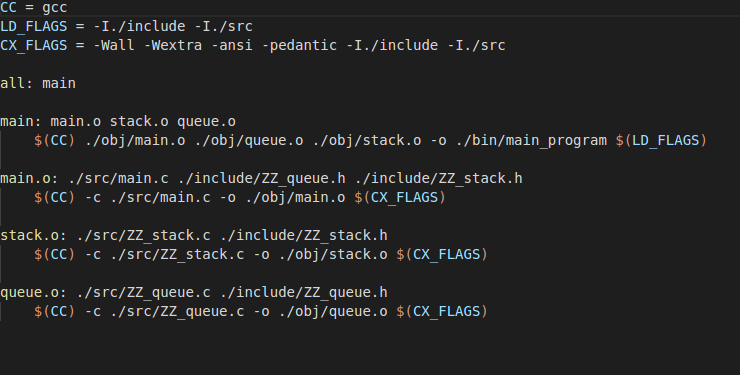
\includegraphics[scale=0.39]{makefile.png}

Makefile
\end{center}

\underline{Jeux de test complets:}
\begin{center}
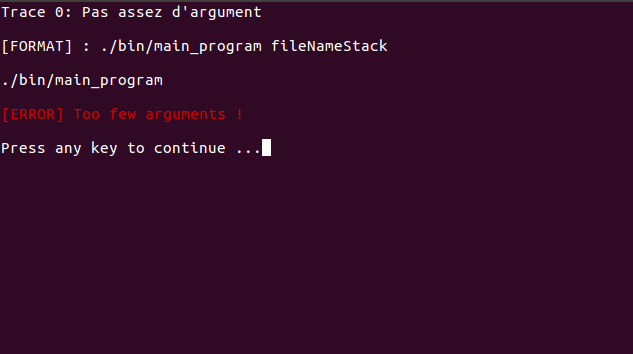
\includegraphics[scale=0.4]{trace0.png}

Terminal 
\end{center}

\begin{center}
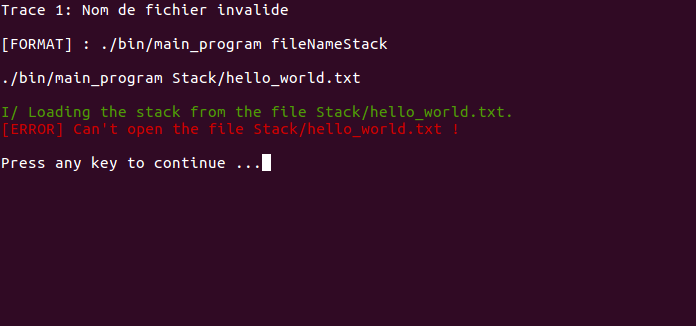
\includegraphics[scale=0.4]{trace1.png}

Terminal
\end{center}

\begin{center}
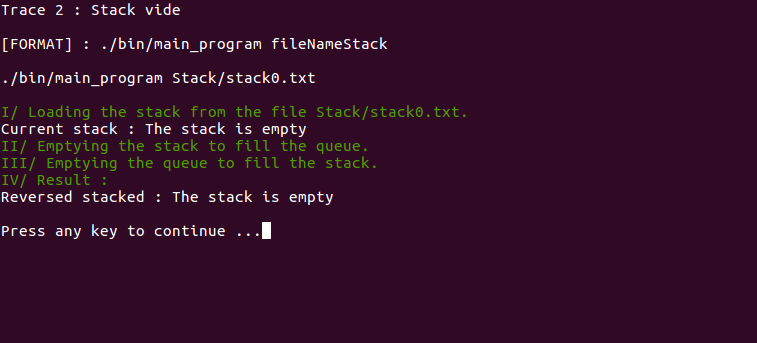
\includegraphics[scale=0.4]{trace2.png}
\fbox{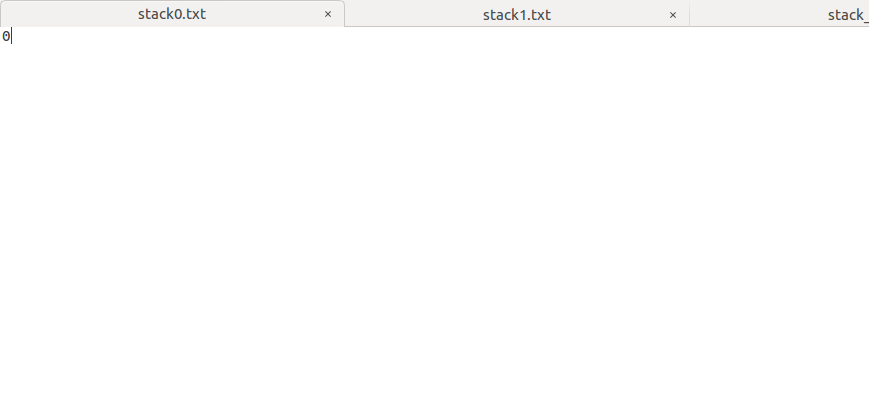
\includegraphics[scale=0.4]{stack_0.png}}

Terminal | fichier pile
\end{center}

\begin{center}
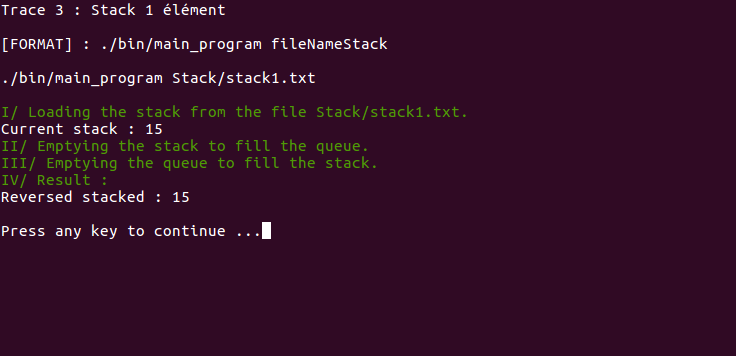
\includegraphics[scale=0.4]{trace3.png}
\fbox{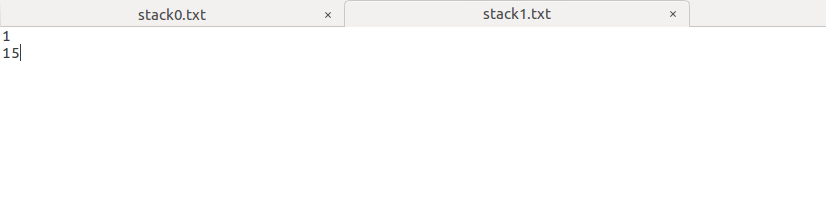
\includegraphics[scale=0.4]{stack1.png}}

Terminal | fichier pile
\end{center}
\begin{center}
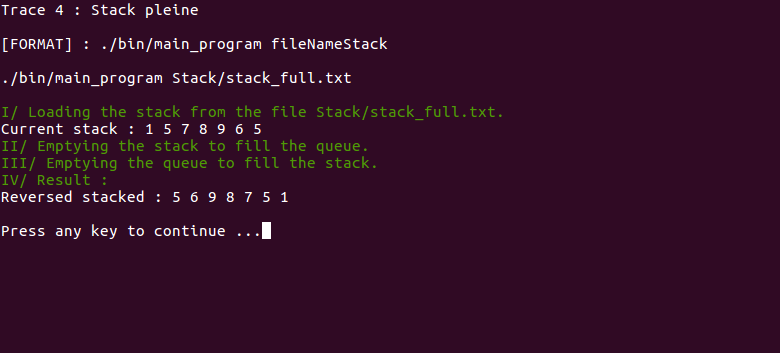
\includegraphics[scale=0.4]{trace4.png}
\fbox{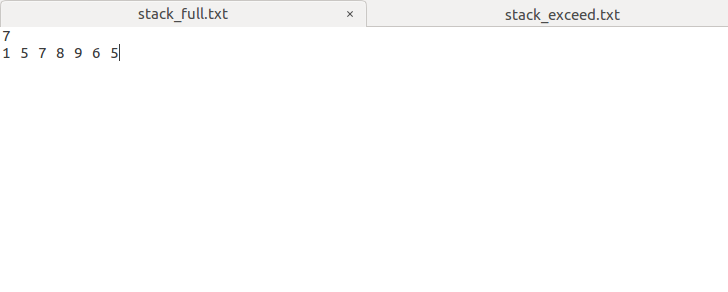
\includegraphics[scale=0.4]{stack_full.png}}

Terminal | fichier pile
\end{center}

\begin{center}
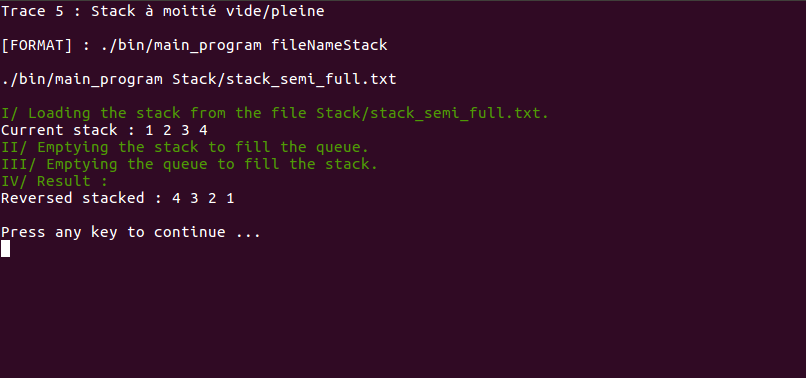
\includegraphics[scale=0.4]{trace5.png}
\fbox{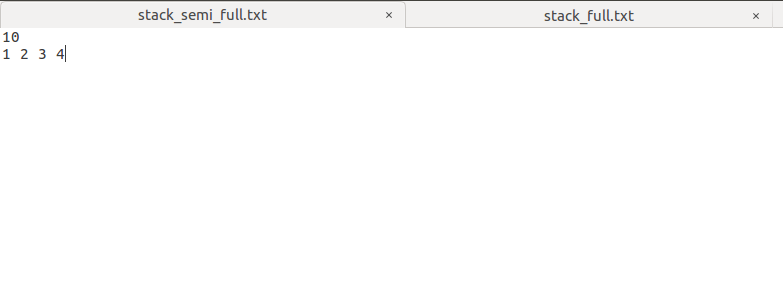
\includegraphics[scale=0.4]{stack_semi_full.png}}

Terminal | fichier pile
\end{center}
\end{document}
